\documentclass[11pt]{article}
\usepackage[margin=1in]{geometry}
\usepackage{volfit_preamble}
\graphicspath{{figures/}}

\title{\textbf{The LQD Model}\\[2pt]
\large A log-quantile-density parametrization for arbitrage-free equity smiles\\[2pt]
\normalsize Vol-Fitter Technical Notes, No.~01}
\author{Vol-Fitter}
\date{\today}

\begin{document}
\maketitle

% Auto-generated by Docs/notes/figures/gen_lqd.py — do not edit.
\newcommand{\lqdoptpts}{2001}
\newcommand{\lqdbarriercenter}{0.90}
\newcommand{\lqdbarrierscale}{50.0}
\newcommand{\lqdsviAL}{0.214458}
\newcommand{\lqdsviAR}{0.069023}
\newcommand{\lqdsvimu}{0.020613}
\newcommand{\lqdsvibetaL}{0.097073}
\newcommand{\lqdsvibetaR}{0.035757}
\newcommand{\lqdsvimaxerr}{0.23}
\newcommand{\lqdsvisigma}{20.62}
\newcommand{\lqdsviskew}{-0.3538}
\newcommand{\lqdsvicurv}{1.6474}
\newcommand{\lqdsvimart}{0.00e+00}
\newcommand{\lqdsvinfev}{7}
\newcommand{\lqdsvicoefftable}{\begin{tabular}{lr} \toprule Parameter & Value\\ \midrule $L$ & -1.87479110\\ $R$ & -3.08957252\\ $a_{2}$ & +0.38076853\\ $a_{3}$ & -0.04700855\\ $a_{4}$ & -0.00719617\\ $a_{5}$ & +0.00645578\\ $a_{6}$ & +0.00213226\\ \bottomrule \end{tabular}}
\newcommand{\lqddhmaxerr}{13.19}
\newcommand{\lqddhAL}{0.015341}
\newcommand{\lqddhAR}{0.014979}
\newcommand{\lqdtimingtable}{\begin{tabular}{rrrrrr} \toprule $N$ & $P$ & analytic (ms) & FD (ms) & speed-up & $|\Delta\mathrm{cost}|$\\ \midrule 6 & 7 & 15.3 & 25.0 & 1.64$\times$ & 5.6e-20\\ 8 & 9 & 20.9 & 29.2 & 1.40$\times$ & 1.4e-19\\ 10 & 11 & 26.6 & 41.7 & 1.57$\times$ & 8.9e-20\\ 12 & 13 & 27.3 & 47.0 & 1.72$\times$ & 2.0e-20\\ \bottomrule \end{tabular}}


\begin{abstract}
This note develops the slice and surface parametrization that the Vol-Fitter calls
\emph{LQD} --- ``log quantile density''. For a single expiry let
$X=\log(S_T/F_T)$ be the log-forward return under the $T$-forward measure, let
$Q(u)$ be its quantile function and $q(u)=Q'(u)$ its quantile density. The model
parametrizes
\[
\ell(u)=\log q(u)=-\log u-\log(1-u)+(1-u)L+uR+\sum_{n=2}^{N}a_nP_n(1-2u),
\qquad u\in(0,1),
\]
where the $P_n$ are Legendre polynomials. The shipped default $N=6$ has seven
parameters (the API supports $4\le N\le16$). Because $q=e^{\ell}>0$ automatically, the recovered
risk-neutral density is non-negative \emph{by construction}: a one-expiry LQD
slice is free of butterfly arbitrage after a single scalar martingale
normalization, with no positivity penalty anywhere in the optimizer. The
logarithmic endpoint terms give exponential return tails, hence linear
implied-variance wings that sit automatically inside Lee's moment bounds; one
explicit integrability condition $A_R<1$ guarantees a finite forward. We give
the full pricing equations, the tail and Lee-slope analysis, the exact
analytic ATM level/skew/curvature handles, the trader-facing ATM-orthogonal
chart, and the calibration objective with its soft tail barrier. A dedicated
section derives the model's \emph{analytic residual Jacobian} --- a clean
cancellation identity that removes the finite-difference quadrature rebuild and
is, to our knowledge, the original engineering contribution of this
implementation. Every figure and table is generated fresh by the production
calibrator on \emph{synthetic approximation benchmarks} (market-fit evidence
lives in the backtest reports): the seven-parameter fit to an SPX-like SVI-JW
target reaches a maximum implied-volatility error of \lqdsvimaxerr\ volatility
basis points, and a thirteen-parameter fit reproduces a bimodal ``double-hat''
event density.
\end{abstract}

\tableofcontents
\newpage

%======================================================================
\section{Purpose and the modelling choice}
\label{sec:purpose}

Most smile models parametrize implied volatility, total variance, or option
price \emph{directly}. That is convenient to quote but awkward to keep
arbitrage-free: non-negativity of the implied risk-neutral density is then a
\emph{global nonlinear} condition on the curve, policed during optimization by
penalties that the fitter can violate on the way to a solution. The LQD model
inverts the construction. It parametrizes a probability law first --- through
the quantile density of the terminal return --- and reads option prices and
implied volatilities off that law by integration afterwards. The design
objective is a single sentence:

\begin{heuristic}
A calibrated slice should be a smooth, flexible smile, yet \emph{every}
admissible parameter vector should already correspond to a genuine probability
law for the terminal forward return. ``Fit a curve, then check it is a
density'' becomes ``fit \emph{within} the space of densities, then read off
implied volatility.''
\end{heuristic}

\begin{invariant}
\begin{enumerate}[leftmargin=1.6em]
\item Every parameter vector prices from a genuine non-negative density:
butterfly-freedom is structural, never a penalty
(\cref{prop:nobutterfly}).
\item The only hard admissibility condition is $A_R<1$ (a finite forward),
guarded by a smooth barrier before the wall.
\item The martingale normalization is a single scalar shift: it changes
neither the density's shape, its tails, nor its positivity.
\item The ATM handles $(\sigma_0,s_0,\kappa_0)$ are exact closed-form
functionals of the slice --- the same three coordinates the graph
extrapolator of Note~14 propagates.
\end{enumerate}
\end{invariant}

The modelling object is the log-forward return
\begin{equation}
X_T=\log\!\left(\frac{S_T}{F_T}\right),
\end{equation}
with $F_T$ the forward for expiry $T$. We suppress discounting and deterministic
carry by working in normalized, undiscounted units; the normalized call at
log-moneyness $k=\log(K/F_T)$ is
\begin{equation}
C_T(k)=\E^{T}\!\left[(e^{X_T}-e^{k})^+\right],
\qquad \E^{T}[e^{X_T}]=1,
\label{eq:call_def}
\end{equation}
the second equality being the martingale (forward) condition. Unless a maturity
is displayed, every formula below is for one expiry.

\paragraph{Time convention.} Three time objects are distinct in production and
must not be conflated: $T$ is the \emph{expiry date}; $t_T$ is its calendar
year fraction; and $\tau_T$ is the \emph{active variance time} --- calendar
time dilated by scheduled events (Note~11), with $\tau_T=t_T$ whenever the
event clock is off or the calendar is empty. Every quantity of the form
$w=\sigma^2\times\text{time}$, every vega, and every ATM-handle annualization
in this note uses $\tau_T$: the calibrator receives \texttt{prepared.tau}, not
the calendar fraction. To keep the classical formulas readable we write a bare
$T$ inside them; wherever $T$ appears in a time role
($w=\sigma^2T$, $\sqrt T$ in a vega, $w_0/T$ in a handle), read $\tau_T$.

\paragraph{Units and vocabulary.} A dollar quote converts to the normalized
units above by $C^{\text{norm}}=C^{\$}/(D_TF_T)$, with $D_T$ the discount
factor to expiry. $\PhiN$ and $\phin$ are the standard normal CDF and PDF. A
\emph{volatility basis point} (vol bp) is $10^{-4}$ in volatility ($0.01$ vol
point). The \emph{(forward Black) delta} of a strike is $\PhiN(d_+)$ --- used
here only as a moneyness label. The \emph{haircut band} is the bid--ask band
shrunk by a fixed vol amount (Note~07). A \emph{risk reversal} (RR) is the
call-minus-put IV difference at matched deltas and a \emph{butterfly} (BF) the
wing-average-minus-ATM IV at matched deltas; both appear only as prior
operators (Note~13). \emph{SVI} is the ``stochastic volatility inspired''
smile parametrization and \emph{SVI-JW} its ``jump-wings'' trader
re-coordinatization (\cref{app:svijw}).

\paragraph{The whole model in one line.} Coefficients
$\theta=(L,R,a_2,\dots,a_N)$ define $g$; integrating $e^{g}$ gives the
quantile $Q$; one scalar shift $\mu$ makes $e^{Q}$ a mean-one law; the
asset-share integral of $e^{Q}$ prices calls; the Black inversion of those
prices is the smile:
\[
\theta\;\to\;g\;\to\;Q\;\to\;\mu\;\to\;C(k)\;\to\;\sigma_{\text{imp}}(k).
\]

If $F_X$ is the law of $X$ and $Q(u)=F_X^{-1}(u)$ for $0<u<1$, the quantile
density is
\begin{equation}
q(u)=Q'(u)=\frac{1}{f_X(Q(u))}.
\end{equation}
Modelling $\ell=\log q$ forces $q>0$, hence $Q$ strictly increasing, hence a
\emph{bona fide} non-negative density. That is the entire structural reason a
one-expiry LQD slice carries no butterfly arbitrage. The chosen basis is
\begin{equation}
\boxed{\;
\ell(u)=-\log u-\log(1-u)+(1-u)L+uR+\sum_{n=2}^{N}a_nP_n(1-2u)\;}
\label{eq:lqd_main}
\end{equation}
and it is deliberately \emph{not} a generic polynomial basis. The two singular
terms $-\log u$ and $-\log(1-u)$ manufacture logarithmic quantile tails ---
equivalently, exponential return tails and therefore the linear
implied-total-variance wings that Lee's formula demands. The endpoint
coefficients $L,R$ scale those tails; the Legendre modes $a_n$ shape the body.
The shipped default $N=6$ carries the seven parameters
$(L,R,a_2,a_3,a_4,a_5,a_6)$; the API accepts $4\le N\le16$, and higher $N$ adds
body detail without ever touching the no-arbitrage mechanism.

In code the positivity is a single line: with the smooth part
$g(u)=(1-u)L+uR+\sum_n a_nP_n(1-2u)$, the return density is $f_X(Q(u))=1/q(u)=
u(1-u)\,e^{-g(u)}$, non-negative for \emph{any} coefficients.

\begin{lstlisting}[caption={The LQD density is structurally non-negative --- no
constraint, no penalty (distilled from \texttt{models/lqd/quadrature.py}).},
label={lst:lqd_density}]
def density(u, g):        # g(u) = (1-u) L + u R + sum a_n P_n(1-2u)
    return u * (1 - u) * np.exp(-g)   # >= 0 for ANY g: no butterfly
\end{lstlisting}

\paragraph{Why this is the right trade.} A direct-IV model spends optimizer
effort \emph{policing} arbitrage; the LQD model spends none, because the feasible
set \emph{is} the set of densities. The price is two scalar nonlinearities: a
martingale normalization (one $\log$ of an integral, \cref{sec:logit}) and a tail
admissibility condition $A_R<1$ (\cref{sec:tails}). Both are cheap, and both are
imposed once per residual evaluation rather than at every quote.

%======================================================================
\section{Static arbitrage and the quantile construction}
\label{sec:static}

\subsection{Normalized prices and Breeden--Litzenberger}

Write $Y=e^X=S_T/F_T$ and let $\widetilde C(y)=\E[(Y-y)^+]$ be the normalized
call as a function of the normalized strike $y=e^k$. A static, butterfly-free
slice requires $\widetilde C$ decreasing and convex in $y$ with
$\widetilde C(0)=1$ and $\widetilde C(\infty)=0$. When $Y$ has a density,
\begin{equation}
\frac{\partial\widetilde C}{\partial y}=-(1-F_Y(y)),
\qquad
\frac{\partial^2\widetilde C}{\partial y^2}=f_Y(y)\ge 0,
\label{eq:BL}
\end{equation}
which is the Breeden--Litzenberger identity: the second strike derivative of the
call \emph{is} the risk-neutral density. The quantile construction supplies such
a density directly. Given a strictly increasing $Q$ for $X$, the quantile of
$Y=e^X$ is $Q_Y(u)=e^{Q(u)}$; if $\int_0^1 e^{Q(u)}\dd u=1$ then $\E[Y]=1$. For
$k\in\R$ let $u_k$ solve $Q(u_k)=k$; then
\begin{align}
C(k)&=\int_{u_k}^1\!\big(e^{Q(u)}-e^{k}\big)\dd u,
\label{eq:call_quantile}\\
P(k)&=\int_0^{u_k}\!\big(e^{k}-e^{Q(u)}\big)\dd u,
\end{align}
and subtracting gives put--call parity $C(k)-P(k)=1-e^k$.

\begin{proposition}[A single LQD slice is butterfly-free]
\label{prop:nobutterfly}
Suppose $q(u)=e^{\ell(u)}>0$ on $(0,1)$ and the martingale integral
$\int_0^1 e^{Q(u)}\dd u$ is finite. After the scalar shift of $Q$ that makes this
integral equal to one, the prices \eqref{eq:call_quantile} are generated by a
probability law on $Y>0$ with mean one; the slice is therefore free of butterfly
arbitrage.
\end{proposition}

\begin{proof}
Since $q>0$, $Q$ is strictly increasing and defines a law for $X$; $Y=e^X>0$;
the shift enforces $\E[Y]=1$. The call is the expectation of $(Y-e^k)^+$ under
this law, so monotonicity and convexity in strike follow from \eqref{eq:BL}. No
separate positivity inequality is ever checked.
\end{proof}

\subsection{The logit coordinate and stable integration}
\label{sec:logit}

The endpoint singularities in \eqref{eq:lqd_main} vanish under the logit change
of variable
\begin{equation}
z=\log\frac{u}{1-u},\qquad u=\Lambda(z)=\frac{1}{1+e^{-z}}.
\end{equation}
Writing the smooth part
$g(u)=(1-u)L+uR+\sum_{n\ge2}a_nP_n(1-2u)$, we have
$q(u)=e^{g(u)}/\big(u(1-u)\big)$ and, crucially,
\begin{equation}
\frac{\dd Q}{\dd z}=q(u)\,u(1-u)=e^{g(\Lambda(z))}.
\label{eq:q_logit}
\end{equation}
All singularities are gone: the quantile is the integral of a smooth positive
function on the line,
\begin{equation}
\overline Q(z)=\int_0^z e^{g(\Lambda(s))}\dd s,
\label{eq:qbar}
\end{equation}
and a scalar shift $\mu$ enforces the martingale constraint,
\begin{equation}
Q(z)=\mu+\overline Q(z),\qquad
\mu=-\log\!\left(\int_{-\infty}^{\infty} e^{\overline Q(z)}\,\Lambda(z)(1-\Lambda(z))\,\dd z\right).
\label{eq:mu_norm}
\end{equation}
This is the \emph{only} normalization; it changes neither $q$, the tails, nor
positivity. Pricing is equally clean. Let $z_k$ solve $Q(z_k)=k$,
$u_k=\Lambda(z_k)$, and define the \emph{upper asset-share integral}
\begin{equation}
A(z)=\int_z^{\infty}e^{Q(s)}\,\Lambda(s)(1-\Lambda(s))\,\dd s.
\label{eq:asset_share}
\end{equation}
Since $1-u_k=\int_{z_k}^{\infty}\Lambda(s)(1-\Lambda(s))\dd s$, the call price is
\begin{equation}
C(k)=A(z_k)-e^{k}(1-u_k).
\label{eq:call_logit}
\end{equation}
A single quadrature grid yields $Q(z)$ and $A(z)$; every strike is then priced by
interpolation. This pricing identity is also the seed of the analytic Jacobian
of \cref{sec:jacobian}, because the implicit dependence of $z_k$ on the
parameters will cancel exactly.

\begin{example}[title={Example: the logistic base --- the whole machine on one toy}]
Set every $a_n=0$ and $L=R=\log s$. Then $g\equiv\log s$, so
\eqref{eq:q_logit} gives $\dd Q/\dd z=s$: the quantile is exactly
$Q(z)=\mu+sz$, i.e.\ $X=\mu+s\log\!\big(U/(1-U)\big)$ is a \emph{logistic} random variable
with scale $s$ and variance $\pi^2s^2/3$. The endpoint scales are
$A_L=A_R=s$, so the slice is admissible iff $s<1$; the shift
\eqref{eq:mu_norm} evaluates to $\mu=-\log\big(\pi s/\sin(\pi s)\big)$ in
closed form; and the smile is a gentle symmetric smile with
$w_0\approx\pi^2s^2/3$. This two-line model is precisely the production
cold-start initializer of \cref{sec:calib}: match $s$ to the ATM variance,
then let the optimizer bend $L\ne R$ (tail asymmetry) and the $a_n$ (body).
\end{example}

%======================================================================
\section{Basis functions and exact coefficients}
\label{sec:basis}

\subsection{The Legendre body}

With $x=1-2u\in(-1,1)$ the Legendre polynomials obey
$\int_{-1}^1 P_mP_n\dd x=\frac{2}{2n+1}\1_{m=n}$, hence
\begin{equation}
\int_0^1 P_m(1-2u)P_n(1-2u)\dd u=\frac{1}{2n+1}\1_{m=n}.
\end{equation}
This is a well-conditioned global basis for the smooth part of $\ell$. The first
two degrees are carried by the endpoint terms, since
\begin{equation}
(1-u)L+uR=\frac{L+R}{2}+\frac{L-R}{2}(1-2u),
\end{equation}
so the seven-parameter $N=6$ model spans the same polynomial space as
$P_0,\dots,P_6$ while preserving the endpoint meaning of the first two
coordinates. The body polynomials are built by the stable three-term recursion
\begin{equation}
(n+1)P_{n+1}(x)=(2n+1)xP_n(x)-nP_{n-1}(x),\qquad P_0=1,\ P_1=x.
\label{eq:leg_recursion}
\end{equation}

\subsection{Endpoint scales}
\label{sec:endpoint}

The endpoint values of $g$ set the tail scales. Because $P_n(1)=1$ and
$P_n(-1)=(-1)^n$,
\begin{align}
A_L&:=e^{g(0)}=\exp\!\Big(L+\textstyle\sum_{n\ge2}a_n\Big),
\label{eq:AL}\\
A_R&:=e^{g(1)}=\exp\!\Big(R+\textstyle\sum_{n\ge2}(-1)^na_n\Big).
\label{eq:AR}
\end{align}
These are not diagnostics --- they are the slopes of the quantile in the logit
coordinate, $Q(z)=\mu+A_Lz+O(1)$ as $z\to-\infty$ and $Q(z)=\mu+A_Rz+O(1)$ as
$z\to+\infty$. The right-tail integrability condition for a \emph{finite forward}
is
\begin{equation}
A_R<1.
\label{eq:AR_condition}
\end{equation}
Indeed, as $z\to+\infty$, $\Lambda(z)(1-\Lambda(z))\sim e^{-z}$ and
$e^{Q(z)}\sim Ce^{A_Rz}$, so the martingale integrand decays like $e^{(A_R-1)z}$,
integrable iff $A_R<1$. On the left the integrand decays like $e^{(A_L+1)z}$ for
every $A_L>0$, so no left condition is needed.

\begin{caution}
$A_R<1$ is a genuine hard constraint, not a regularization preference: an LQD
slice with $A_R\ge1$ has an \emph{infinite} forward and its ``prices'' are
meaningless. The calibrator enforces it with a hard rejection \emph{and} a smooth
soft barrier that engages well before the boundary (\cref{sec:calib}), so the
finite-difference and analytic Jacobians stay smooth as the optimizer approaches
the wall.
\end{caution}

%======================================================================
\section{Tail asymptotics and Lee moment boundaries}
\label{sec:tails}

\subsection{Return moments}

The endpoint linearity of $Q$ in $z$ gives exponential return tails. For large
$x$, $z\sim x/A_R$ and $1-u\sim e^{-z}$, so
\begin{equation}
\Q(X>x)\asymp e^{-x/A_R},\qquad x\to+\infty,
\end{equation}
and symmetrically $\Q(X<x)\asymp e^{x/A_L}$ as $x\to-\infty$. The moment
generating function of $X$ therefore has critical strip
$-1/A_L<r<1/A_R$, and since $Y=e^X$ has mean one,
\begin{equation}
p_R^*=\sup\{p\ge0:\E[Y^{1+p}]<\infty\}=\frac{1}{A_R}-1,
\qquad
q_L^*=\sup\{q\ge0:\E[Y^{-q}]<\infty\}=\frac{1}{A_L}.
\label{eq:critical}
\end{equation}

\subsection{Lee wing slopes}

Let $w(k,T)=\sigma_{\BS}^2(k,T)\,T$ be total implied variance. Lee's moment
formula gives the asymptotic total-variance slopes
$\beta_R=\limsup_{k\to+\infty}w/k$ and
$\beta_L=\limsup_{k\to-\infty}w/|k|$ as
\begin{equation}
\beta=\psi(p),\qquad \psi(p)=2-4\big(\sqrt{p^2+p}-p\big),
\qquad p\in[0,\infty],
\label{eq:lee_psi}
\end{equation}
equivalently $\tfrac{1}{2\beta}+\tfrac{\beta}{8}-\tfrac12=p$, $0<\beta\le2$.
Combining with \eqref{eq:critical},
\begin{equation}
\beta_L=\psi\!\left(\frac{1}{A_L}\right),
\qquad
\beta_R=\psi\!\left(\frac{1}{A_R}-1\right),\quad A_R<1.
\label{eq:lee_slopes}
\end{equation}
The endpoint coefficients thus do double duty: they regularize extrapolation
\emph{and} identify the moment critical exponents and the Lee-consistent wing
slopes. A calibration may fit $L,R$ freely (subject only to $A_R<1$) or impose
explicit wing priors by constraining $A_L,A_R$ through
\eqref{eq:AL}--\eqref{eq:AR}. The cross-model treatment of wings and Lee bounds
is the subject of Note~09; here they fall out of the parametrization for free.

\begin{heuristic}
The map $\psi$ is decreasing: a \emph{heavier} tail (larger $A$, hence smaller
critical exponent) gives a \emph{steeper} variance wing (larger $\beta$). Be
precise about ``fat'': LQD return tails are \emph{exponential}, hence
asymptotically \emph{much} heavier than the log-normal's Gaussian log-return
tails --- though over traded strikes the two can look close. Equity index
smiles fit small $A_L,A_R$, so their wings sit comfortably below the
model-free ceiling $\beta=2$, and a truncation $z\in[-40,40]$ in double
precision is far more than enough (\cref{sec:quadrature}).
\end{heuristic}

%======================================================================
\section{Option pricing and implied-volatility recovery}
\label{sec:pricing}

\subsection{The Black map and vega-normalized residuals}

The normalized Black call in total-variance units is
\begin{equation}
\Black(k,w)=\PhiN(d_+)-e^{k}\PhiN(d_-),\qquad
d_\pm=-\frac{k}{\sqrt w}\pm\frac{\sqrt w}{2},
\label{eq:black}
\end{equation}
and the implied total variance generated by the slice solves
$\Black(k,w(k,T))=C_T(k)$. For calibration the loss is expressed in vega-scaled
price units rather than raw price, so that it approximates a volatility error
while preserving the exact arbitrage-free price construction during the solve:
given quoted volatility $\sigma_i$ at $k_i$, with $w_i=\sigma_i^2T$,
\begin{equation}
r_i(\theta)=\frac{C^{\mathrm{LQD}}(k_i;\theta)-\Black(k_i,w_i)}{\partial_\sigma \Black(k_i,w_i)+\eta},
\qquad \partial_\sigma\Black=\phin(d_+)\sqrt T,
\label{eq:vega_resid}
\end{equation}
with a small floor $\eta$ in the far wings (\cref{app:atlas}, $\eta=$
\texttt{\_VEGA\_FLOOR}). Working in price space keeps every iterate a valid
density; the vega division undoes the price-to-vol scale so the optimizer sees
something close to a vol residual.

\subsection{Quadrature, Hermite interpolation, and Newton inversion}
\label{sec:quadrature}

On a finite logit grid $z_j\in[-Z,Z]$ the pipeline computes, in one pass,
$u_j=\Lambda(z_j)$, $h_j=e^{g(u_j)}$, the cumulative $\overline Q_j$ by
(fourth-order) cumulative Simpson quadrature, the shift $\mu$ from
\eqref{eq:mu_norm}, and the reverse-cumulative asset share $A_j$. The two
truncation tails are added analytically: at the right,
\begin{equation}
\int_Z^{\infty}e^{Q}\Lambda(1-\Lambda)\dd z\approx\frac{e^{Q(Z)-Z}}{1-A_R},
\qquad
\int_{-\infty}^{-Z}e^{Q}\Lambda(1-\Lambda)\dd z\approx\frac{e^{Q(-Z)-Z}}{1+A_L}.
\label{eq:tail_corr}
\end{equation}
For equity tails with $A_L,A_R$ small, $Z=40$ buries the truncation error far
below double-precision vega noise.

Two implementation refinements matter for accuracy and for the analytic
Jacobian. First, the production build stores the \emph{exact nodal derivatives}
$\dd Q/\dd z=e^{g}$ and $\dd A/\dd z=-e^{Q}u(1-u)$ alongside the nodal values, so
both $Q$ and $A$ are interpolated off-grid with \emph{cubic Hermite}
polynomials, not linear interpolation. Priced curves are then smooth enough for
clean finite-difference Greeks, and --- because Hermite interpolation returns the
nodal value exactly at a node --- calendar constraints expressed at grid
$z$-values match node-indexed ones bit-for-bit. Second, the strike inversion
$Q(z_k)=k$ is solved by \emph{Hermite--Newton} iteration to machine precision,
not by a coarse table lookup, which keeps the ATM handles (\cref{sec:atm})
exact.

\begin{perfbox}
The quadrature grid $(z,u,u(1-u))$ and the Legendre matrix $P_n(1-2u)$ depend
only on $(Z,n_{\text{pts}})$ and the model order --- never on $\theta$. A single
calibration builds the slice many hundreds of times, so these arrays are cached
(returned read-only) and only the parameter-dependent combination $g(u)$ is
re-formed per call; this alone made \texttt{build\_slice} about $1.7\times$
faster. Optimization runs on a coarser $n_{\text{pts}}=\lqdoptpts$ grid whose
Simpson error is already orders of magnitude below the fit budget, and the
\emph{accepted} slice is rebuilt once at the full grid for reporting, density,
var-swap and calendar diagnostics. See \cref{app:perf}.
\end{perfbox}

%======================================================================
\section{Exact ATM handles and the orthogonal chart}
\label{sec:atm}

\subsection{Level, skew and curvature from the quantile}
\label{sec:atm_exact}

Traders want the first coordinates of a model to be \emph{actual} ATM level,
skew and curvature. The LQD slice delivers these in closed form, with no finite
differencing of implied volatility. Let $u_0$ solve $Q(u_0)=0$, set
$c_0=C(0)$, and let $f_0=f_X(0)=u_0(1-u_0)e^{-g(u_0)}$ be the ATM return density.
The first two \emph{log-strike} call derivatives are exactly
\begin{equation}
C'(0)=-(1-u_0),\qquad C''(0)=f_0-(1-u_0),
\label{eq:Cder}
\end{equation}
where $C''$ is in log-strike (from $C'(k)=-e^{k}(1-F_X(k))$). Let $w_0$ solve the
ATM Black identity $\Black(0,w_0)=2\PhiN(\sqrt{w_0}/2)-1=c_0$. With $a=\sqrt{w_0}/2$,
$n=\phin(a)$, $\PhiN_a=\PhiN(a)$, the Black partials at $k=0$ are
\begin{equation}
\begin{aligned}
\Black_k&=-(1-\PhiN_a), &
\Black_w&=\tfrac{n}{2\sqrt{w_0}}, &
\Black_{kk}&=-(1-\PhiN_a)+\tfrac{n}{\sqrt{w_0}},\\
\Black_{kw}&=\tfrac{n}{4\sqrt{w_0}}, &
\Black_{ww}&=-\tfrac{n}{4w_0^{3/2}}-\tfrac{n}{16\sqrt{w_0}}. & &
\end{aligned}
\end{equation}
Differentiating $\Black(k,w(k))=C(k)$ once and twice at $k=0$ gives
\begin{equation}
w_1=\frac{C'(0)-\Black_k}{\Black_w},
\qquad
w_2=\frac{C''(0)-\Black_{kk}-2\Black_{kw}w_1-\Black_{ww}w_1^2}{\Black_w},
\end{equation}
and the actual implied-volatility handles are
\begin{equation}
\sigma_0=\sqrt{\tfrac{w_0}{T}},\quad
s_0=\frac{w_1}{2\sqrt{Tw_0}},\quad
\kappa_0=\frac{w_2}{2\sqrt{Tw_0}}-\frac{w_1^2}{4\sqrt{T}\,w_0^{3/2}}.
\label{eq:atm_handles}
\end{equation}
These are exact for every LQD slice, and their meaning and units are worth
stating: $\sigma_0=\sigma_{\text{imp}}(0)$ is the ATM implied volatility
(annualized on the active clock $\tau_T$),
$s_0=\partial_k\sigma_{\text{imp}}(0)$ is the ATM \emph{skew} (volatility per
unit log-moneyness) and $\kappa_0=\partial_{kk}\sigma_{\text{imp}}(0)$ the ATM
\emph{curvature} (volatility per unit log-moneyness squared). Two closely
related coordinate triples coexist in production and must not be conflated:
the \emph{graph-facing carrier} is $h=(\sigma_0,s_0,\kappa_0)$ --- what
Note~14 propagates across the smile graph --- while the \emph{internal
orthogonal chart} of \cref{sec:ortho} works in $H=(w_0,s_0,\kappa_0)$ with
$w_0=\sigma_0^2\,\tau_T$ the ATM total variance (\texttt{models/lqd/ortho.py};
the graph adapter converts between the two).

\subsection{The ATM-orthogonal chart}
\label{sec:ortho}

Collect the three handles into $H(\theta)=(w_0,s_0,\kappa_0)$ --- note the
first coordinate is the ATM \emph{total variance}, not $\sigma_0$
(\cref{sec:atm_exact}) --- and let
$J=\partial H/\partial\theta\in\R^{3\times d}$ at a reference $\theta^*$ (computed
by central differences; the quadrature is deterministic, so this is accurate to
$\sim10^{-9}$). The least-norm perturbation realizing a desired handle change
$\delta h$ is $\delta\theta=J\T(JJ\T)^{-1}\delta h$, and
$\Pi_\perp=I-J\T(JJ\T)^{-1}J$ projects onto handle-preserving directions. With
$U=J\T(JJ\T)^{-1}$ (so $JU=I_3$) and $V$ an orthonormal basis of $\ker J$ from the
QR factorization of $\Pi_\perp$, the chart
\begin{equation}
\theta=\theta^*+U\alpha+V\xi
\end{equation}
has \emph{three primary coordinates} $\alpha$ that move the trader handles and
\emph{shape coordinates} $\xi$ that leave them fixed to first order. For larger
moves the map is made exact by a three-dimensional Newton solve of
$H(\theta^*+U\alpha+V\xi)=h^{\text{target}}$ (the ``retarget''); because $JU=I_3$
the $3\times3$ Jacobian is the identity at the reference, an excellent
preconditioner that rarely needs refreshing. This is what lets a trader drag ATM
level, skew or curvature while the optimizer keeps using the remaining Legendre
modes for wings, shoulders and event convexity.

\begin{caution}
The chart is \emph{local}: $U$ and $V$ are built from the Jacobian at the
reference $\theta^*$, so the first-order handle-invariance of the shape
directions degrades for large excursions, and the retarget Newton solve can
fail to converge --- or converge only to an \emph{infeasible} point --- when
the requested handles push the slice toward the $A_R=1$ integrability wall
(e.g.\ a large curvature move on a thin-tailed reference). Callers must treat
retargeting as an operation that can fail near the wall, not as a total map on
handle space.
\end{caution}

%======================================================================
\section{Calibration of one expiry}
\label{sec:calib}

\subsection{The objective}

Given quotes $(k_i,\sigma_i,\omega_i)$ at one maturity, with $w_i=T\sigma_i^2$,
the calibrator minimizes
\begin{equation}
\min_\theta\;\sum_i\omega_i\!\left(\frac{C^{\mathrm{LQD}}(k_i;\theta)-\Black(k_i,w_i)}{\partial_\sigma\Black(k_i,w_i)+\eta}\right)^{\!2}
+\lambda\sum_{n\ge4}n^{2r}a_n^2,
\label{eq:calib_objective}
\end{equation}
as a bound-free nonlinear least-squares problem (scipy \texttt{trf}). The
high-order ridge $\lambda\,n^{2r}a_n^2$ is optional and suppresses oscillation in
sparse markets; it deliberately leaves the first body modes $a_2,a_3$ free. The
hard admissibility condition is $A_R<1-\eps_R$ for a small buffer $\eps_R$. There
is \emph{no} density-positivity term --- positivity is structural
(\cref{prop:nobutterfly}). Equation~\eqref{eq:calib_objective} shows only the
\emph{core} rows (data $+$ ridge); the full production residual stack, with each
block's activation condition and Jacobian route, is tabulated in
\cref{sec:hooks}.

\paragraph{The soft tail barrier.} To keep the residual smooth as the optimizer
approaches the $A_R=1$ wall, the stacked residual carries a softplus barrier
\begin{equation}
b(\theta)=\log\!\big(1+e^{\,s(A_R-c)}\big),
\label{eq:barrier}
\end{equation}
with centre $c=$ \lqdbarriercenter\ and steepness $s=$ \lqdbarrierscale\ (both
\texttt{FitSettings} coefficients; evaluated as
$\operatorname{logaddexp}(0,\cdot)$ so a wild trial $\theta$ cannot overflow
it). The barrier is negligible for $A_R\ll c$ and
rises steeply near the wall, pushing the fit back \emph{before} it reaches the
hard rejection. When a trial $\theta$ does cross $A_R\ge1$, the price block is
replaced by a large smooth-in-$A_R$ penalty $10+A_R$ so the trust region still
has a gradient pointing back to feasibility.

\subsection{Initialization}

The cold-start initializer is the \emph{logistic base}: $a_n=0$, $L=R=\log s$
with $s=\sqrt{3w_0}/\pi$ from the variance match $\Var(X)=\pi^2s^2/3$, seeded
from the ATM-interpolated quote variance --- the \texttt{logistic\_init}
routine of \texttt{calibrate.py}, and exactly the toy of the example in
\cref{sec:logit}. It is the only cold initializer in production. Sequential
workflows do better than cold: the background Calibrate sweep \emph{warm-starts}
each expiry from the previous, shorter-dated expiry's freshly fitted
parameters (adjacent maturities have nearly the same smile, so \texttt{trf}
lands close to the optimum), and the service can also run a \emph{data-only
prepass} --- a persistence-free fit used as the measurement stage of the prior
and filter machinery (Notes~13, 15). Wing-aware and quantile-projection
initializers are roadmap items, not shipped code.

\subsection{The full residual stack}
\label{sec:hooks}

The production objective is the stacked residual of
\cref{tab:stack} --- \texttt{calibrate\_slice} concatenates, in order: the
data block, the ridge, the calendar slack, the barrier, and the optional
var-swap/prior blocks. Every optional block is byte-identical-to-absent when
unused (test-locked), and each connects this note to the rest of the series.
The Jacobian column matters operationally: the analytic route of
\cref{sec:jacobian} covers the first five blocks; activating \emph{any}
var-swap or prior block switches the whole fit to scipy's finite-difference
Jacobian (correct, merely not accelerated).

\begin{table}[H]
\centering\small
\setlength{\tabcolsep}{4pt}
\begin{tabular}{@{}p{0.24\textwidth}p{0.26\textwidth}p{0.24\textwidth}l@{}}
\toprule
Residual block & Active when & Units / scaling & Jacobian\\
\midrule
Mid data block & \texttt{fitMode=mid} (default) & vega-normalized price
($\approx$ vol) & analytic\\
Band data block (hinge $+$ mid anchor; Note~07) & \texttt{fitMode}
\texttt{bidask}/\texttt{haircut} & vega-normalized price & analytic\\
High-order ridge & \texttt{regLambda}$>0$ (rows $n\ge4$) & coefficient units &
analytic\\
Calendar slack (Note~10) & \texttt{enforceCalendar} $+$ a nearer fitted expiry
& asset share (normalized price) & analytic\\
$A_R$ soft barrier & always (one row) & dimensionless & analytic\\
\midrule
Market var-swap (Note~08) & \texttt{varSwapEnabled} $+$ an active quote &
vol & FD fallback\\
Prior strike-gap anchor (Note~13) & \texttt{strike\_gap} / \texttt{hybrid}
tail, active prior & vega-normalized price & FD fallback\\
Prior var-swap companion (Note~13) & alongside an active prior & vol & FD
fallback\\
Operator prior (Note~13) & \texttt{quote\_operator} / \texttt{hybrid}, gated
per operator & operator units (vol) & FD fallback\\
Active-filter MAP (Note~15) & filter mode \texttt{active} (rides the operator
block, ungated) & handle units & FD fallback\\
\bottomrule
\end{tabular}
\caption{The LQD residual stack as production assembles it
(\texttt{models/lqd/calibrate.py}; the prior/filter targets are resolved in
\texttt{api/service.py}). ``FD fallback'' means the presence of that block
switches the entire fit to the finite-difference Jacobian.}
\label{tab:stack}
\end{table}

\subsection{The var-swap route: a native log-contract quadrature}
\label{sec:varswap}

The log-contract identity $w_{\text{vs}}=-2\,\E[X]=-2\int_0^1 Q(u)\dd u$ is
exact for the log-contract \emph{proxy} of the var swap; LQD evaluates it as a
single trapezoidal quadrature on the grid it already owns,
\begin{equation}
w_{\text{vs}}=-2\int_{-\infty}^{\infty}Q(z)\,\Lambda(z)(1-\Lambda(z))\,\dd z,
\end{equation}
whose integrand decays like $z\,e^{-|z|}$
(\texttt{quadrature.py::var\_swap\_strike}). Two qualifications keep the claim
honest. First, this is a \emph{direct native one-dimensional quadrature},
dramatically cheaper than the generic strike replication of Note~08 --- which
would re-solve implied variance on a strike grid at every Jacobian column and
turn a millisecond fit into minutes --- but activating the var-swap block also
disables the analytic Jacobian (\cref{tab:stack}), so a var-swap fit is
\emph{not} literally as cheap as a mid fit. Second, the identity prices the
log contract: its correspondence with a realized-variance swap assumes the
continuous-monitoring, continuous-path (diffusion) convention; jumps and
discrete sampling require the usual corrections, which are outside this
model's scope.

%======================================================================
\section{The analytic residual Jacobian}
\label{sec:jacobian}

The dominant cost of \eqref{eq:calib_objective} used to be the Jacobian: scipy
rebuilt the entire quadrature pipeline $P+1$ times per iteration to finite
difference it ($P=d=N+1$ parameters). The Vol-Fitter instead propagates the
analytic Jacobian of the \emph{core} residual stack --- the mid or band data
block, ridge, calendar slack and barrier rows of \cref{tab:stack} --- in
\emph{one} quadrature pass; a fit with any var-swap or prior block active falls
back to finite differences. The key is a cancellation identity, and it is the
cleanest piece of mathematics in the implementation.

\subsection{The cancellation identity}

Regard the priced call \eqref{eq:call_logit} as a function of $\theta$ through
both the slice and the strike root $z_k(\theta)$ that solves $Q(z_k;\theta)=k$:
\begin{equation}
C(k;\theta)=A(z_k;\theta)-e^{k}\big(1-\Lambda(z_k)\big).
\end{equation}
Differentiating,
\begin{equation}
\frac{\dd C}{\dd\theta}
=\underbrace{\frac{\partial A}{\partial\theta}\Big|_{z}}_{\text{explicit}}
+\Big[\,\underbrace{A_z(z_k)}_{=-e^{Q(z_k)}\Lambda(1-\Lambda)}
+\,e^{k}\Lambda'(z_k)\Big]\frac{\dd z_k}{\dd\theta}.
\end{equation}
Now $A_z(z)=-e^{Q(z)}\Lambda(z)(1-\Lambda(z))$ from \eqref{eq:asset_share}, and at
$z_k$ we have $e^{Q(z_k)}=e^{k}$ and $\Lambda'(z_k)=\Lambda(1-\Lambda)=u_k(1-u_k)$.
Hence the bracket is
\begin{equation}
A_z(z_k)+e^{k}\Lambda'(z_k)
=-e^{k}u_k(1-u_k)+e^{k}u_k(1-u_k)=0.
\end{equation}

\begin{theorem}[Implicit-root cancellation]
\label{thm:cancel}
The implicit dependence of the strike root $z_k$ on the parameters drops out of
the price gradient, leaving
\begin{equation}
\frac{\dd C}{\dd\theta}
=\left.\frac{\partial A}{\partial\theta}\right|_{z=z_k}.
\label{eq:dC}
\end{equation}
\end{theorem}

\noindent So $\dd C/\dd\theta$ is obtained by evaluating the \emph{nodal}
parameter-sensitivities of the asset share at the fixed point $z_k$ --- by the
very same Hermite interpolation used to price, fed the nodal sensitivities
$\partial A/\partial\theta_j$ and $\partial A_z/\partial\theta_j$ instead of the
nodal values.

One honesty note on exactness. \Cref{thm:cancel} is exact for the
\emph{continuous} objects. The production discretization interpolates $Q$ and
$A$ as two separate Hermite interpolants, so between grid nodes the
interpolated price is not \emph{algebraically} the integral of the
interpolated quantile, and the implemented gradient inherits that (tiny)
discretization mismatch. The operational claim is therefore \emph{benchmarked
numerical agreement}, not algebraic identity: the analytic Jacobian matches a
3-point finite difference to a relative $10^{-3}$ tolerance on the mid, band
and calendar stacks, and analytic and finite-difference \emph{fits} reach the
same solution ($|\Delta\theta|\lesssim10^{-5}$, cost agreement
$\sim10^{-11}$; \texttt{test\_lqd\_jacobian.py}).

\subsection{Nodal sensitivities}

Everything reduces to differentiating \eqref{eq:qbar}--\eqref{eq:asset_share}
term by term, using that $g$ is \emph{affine} in $\theta$ with constant basis
$\phi_j=\partial g/\partial\theta_j$ --- namely $\phi_L=1-u$, $\phi_R=u$ and
$\phi_{a_n}=P_n(1-2u)$. Since $\overline Q'=e^{g}$,
\begin{equation}
\frac{\partial\overline Q(z)}{\partial\theta_j}
=\int_0^z e^{g(\Lambda(s))}\phi_j(\Lambda(s))\,\dd s,
\end{equation}
again by cumulative quadrature, anchored at the centre node. The martingale shift
$\mu=-\log M$ with $M=\int e^{\overline Q}\Lambda(1-\Lambda)\dd z$ differentiates to
\begin{equation}
\frac{\partial\mu}{\partial\theta_j}=-\frac{1}{M}\int e^{\overline Q}\,\frac{\partial\overline Q}{\partial\theta_j}\,\Lambda(1-\Lambda)\,\dd z
\;+\;(\text{the two analytic tail-correction terms}),
\end{equation}
where the tail corrections \eqref{eq:tail_corr} contribute their own
$\theta$-derivatives through $\overline Q(\pm Z)$ and through $A_L,A_R$ (whose
gradients are $A_L\,(\1,0,\1\ldots)$ and $A_R\,(0,\1,(-1)^n\ldots)$ from
\eqref{eq:AL}--\eqref{eq:AR}). Then $\partial Q/\partial\theta_j=\partial\mu/\partial\theta_j+\partial\overline Q/\partial\theta_j$,
the asset-share sensitivity follows by reverse cumulative quadrature of
$\partial(e^{Q}u(1-u))/\partial\theta_j$ plus its right-tail correction, and the
nodal $\partial A_z/\partial\theta_j$ is just $-\partial(e^{Q}u(1-u))/\partial\theta_j$.
The remaining residual blocks differentiate trivially: the band hinge multiplies
$\dd C/\dd\theta$ by the violation sign, the ridge block is $\diag(\text{reg})$ on
the $a$-columns, the calendar slack is $\sqrt{\text{cal wt}}\,(-\dd A/\dd\theta)$
on the active constraints, and the barrier row is
$\expit\!\big(s(A_R-c)\big)\,s\,\partial A_R/\partial\theta$.

\subsection{Scope and measured speed-up}

The analytic Jacobian covers the configuration with \emph{no} var-swap or prior
blocks (the var-swap and prior-anchor terms are not yet differentiated
analytically; those fits fall back to scipy's two-point finite difference ---
correct, merely not accelerated). \Cref{tab:timing} reports a fresh comparison:
the analytic and finite-difference fits reach the same fitted solution within
the stated tolerances (costs agreeing to $\sim11$ significant figures,
relative difference $\sim10^{-11}$) while the analytic Jacobian is
$1.3$--$1.7\times$ faster across $N=6\ldots12$ on this benchmark, with both
paths converging in a handful of iterations. Scope of the measurement: the
generator times the least-squares \emph{residual path} (repeated
\texttt{calibrate\_slice} calls on the synthetic benchmark), not the full
public calibration-and-reporting workflow; it runs single-threaded on this
development machine with the static-grid cache warm and only the core residual
blocks active. Different hardware, cache state or an active var-swap/prior
block will move the ratio.

\begin{table}[H]
\centering
\caption{Analytic vs.\ two-point finite-difference Jacobian, fresh run of the
production calibrator on the SVI-JW benchmark (fastest of three repeats,
single-threaded, warm static-grid cache, core residual blocks only). $P=N+1$
is the parameter count; the cost column confirms the same optimum within
tolerance.}
\label{tab:timing}
\lqdtimingtable
\end{table}

\begin{heuristic}
Why only $\sim1.5\times$ and not $\sim P\times$? Two reasons. First, the cached
static grid makes a \emph{repeat} \texttt{build\_slice} cheap, so the $P+1$
finite-difference builds are not $P+1$ times the cost of one cold build. Second,
\texttt{trf} converges here in $\sim7$ iterations, so the linear algebra and the
single value evaluation dilute the Jacobian saving. The win is larger on heavier
configurations, and the benchmark reaches the same fitted solution within the
stated tolerances. The structural payoff --- a Jacobian that no longer rebuilds
the quadrature --- is what makes higher-order and surface-wide fits comfortable.
\end{heuristic}

%======================================================================
\section{Soft calendar-arbitrage control}
\label{sec:calendar}

\Cref{prop:nobutterfly} kills butterfly arbitrage within a slice but says nothing
across expiries. Two standing assumptions frame this section: carry is
deterministic (so working under each $T$-forward measure in normalized units is
legitimate) and every slice is normalized to mean one, $\E[Y_T]=1$. For
$T_1<\dots<T_M$, absence of calendar arbitrage at fixed log-moneyness is
$C_{T_i}(k)\le C_{T_j}(k)$ for $T_i<T_j$ --- equivalently the laws of $Y_T$
increase in \emph{convex order}. In plain language: the longer-dated law is
``more spread out'' --- every convex payoff (every call, at every strike) is
worth at least as much under it --- without its mean moving. With equal means,
$Y_{T_i}\le_{cx}Y_{T_j}$ iff the \emph{integrated upper-quantile} curves are
ordered,
\begin{equation}
G_i(\alpha):=\int_\alpha^1 e^{Q_i(u)}\dd u\;\le\;G_j(\alpha)\quad\forall\alpha\in[0,1],
\label{eq:calendar}
\end{equation}
with equality at $\alpha=0$. This is exactly the upper asset share of
\eqref{eq:asset_share} read at quantile level, so it is already on the grid. The
surface is built nearest-to-farthest: each new slice is fitted subject to
$G_i(\alpha_m)\ge G_{i-1}(\alpha_m)-\eps_m$ on a dense $\alpha$-grid, where
$\eps_m\ge0$ is a per-node slack tolerance --- production currently runs
$\eps_m=0$ (no tolerance) --- enforced as the soft calendar slack of
\eqref{eq:calib_objective} (penalty weight \texttt{calendarWeight}), with the
constraint evaluated at $z$-values so it is exact regardless of the
optimization grid. The quantile constraint is better conditioned than a grid of
call inequalities because it never inverts $Q$ at a strike and stays meaningful
in the wings where IV inversion is ill-conditioned.

Honesty about the guarantee: this is \emph{control}, not a theorem. The hinge
carries a finite weight, so a hard-pressed fit can retain a small violation
rather than destroy the quote fit; the whole coupling is a user toggle
(\texttt{enforceCalendar}) and off means off; and residual calendar violations
are \emph{measured and reported} by the surface diagnostics rather than assumed
away. Note~10 develops the model-agnostic calendar machinery (and the subtlety
that the variance floor must be confined to the traded log-$k$ range); here we
only record that for LQD the constraint is the native object $A(z)$.

%======================================================================
\section{Worked examples}
\label{sec:examples}

All numbers and figures in this section are produced by
\texttt{Docs/notes/figures/gen\_lqd.py}, which fits the production calibrator to
two synthetic targets. Read them for what they are: \emph{synthetic
approximation benchmarks} --- they measure how well the basis can reproduce a
known clean curve, not how well the model fits noisy market quotes.
Market-fit evidence (RMS vs bid--ask NBBO quotes, in- and out-of-sample,
against an SVI-JW baseline) lives in the backtest harness and its reports
(\texttt{backend/backtest/}).

\subsection{An SPX-like SVI-JW smile}

The benchmark target is a six-month SPX-like slice from raw SVI
$w(k)=a+b\{\rho(k-m)+\sqrt{(k-m)^2+\sigma_{\mathrm{SVI}}^2}\}$ with
\begin{equation*}
(a,\,b,\,\rho,\,m,\,\sigma_{\mathrm{SVI}})
=(0.010625,\;0.07289,\;-0.5,\;0.05831,\;0.10100),
\end{equation*}
an ATM
volatility near $20.6\%$ with a pronounced index put skew. The seven-parameter
$N=6$ fit over $k\in[-0.35,0.30]$ converges in \lqdsvinfev\ residual evaluations
to the coefficients of \cref{tab:svi_coeffs}, with endpoint and Lee diagnostics
\begin{equation}
A_L=\lqdsviAL,\quad A_R=\lqdsviAR,\quad \mu=\lqdsvimu,\quad
\beta_L=\lqdsvibetaL,\quad \beta_R=\lqdsvibetaR.
\end{equation}
For comparison the raw-SVI wing slopes are $b(1-\rho)=0.1093$ (left) and
$b(1+\rho)=0.0364$ (right): the Lee slopes agree to $\sim$2 digits on the right
wing ($\beta_R=\lqdsvibetaR$ vs $0.0364$) and to $\sim$1 on the steeper left
($\beta_L=\lqdsvibetaL$ vs $0.1093$, $\sim$10\%), even though nothing imposed it
--- they emerge from the fitted endpoint basis. The exact ATM
handles are $\sigma_0=\lqdsvisigma\%$, $s_0=\lqdsviskew$, $\kappa_0=\lqdsvicurv$,
and the martingale check returns $\E[e^X]-1=\lqdsvimart$. The maximum
implied-volatility error over the calibration grid is \lqdsvimaxerr\ volatility
basis points (\cref{fig:svi}) --- an approximation-capacity number on a clean
synthetic target, not a market-fit error.

\begin{figure}[H]
\centering
\begin{minipage}{0.49\textwidth}\centering
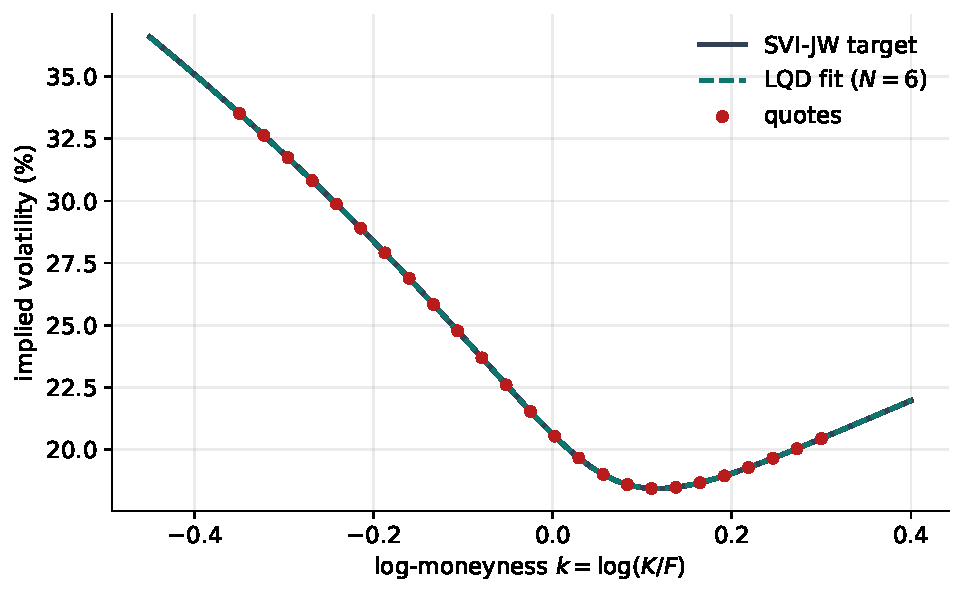
\includegraphics[width=\textwidth]{fig_lqd_svi_fit.pdf}
\end{minipage}\hfill
\begin{minipage}{0.49\textwidth}\centering
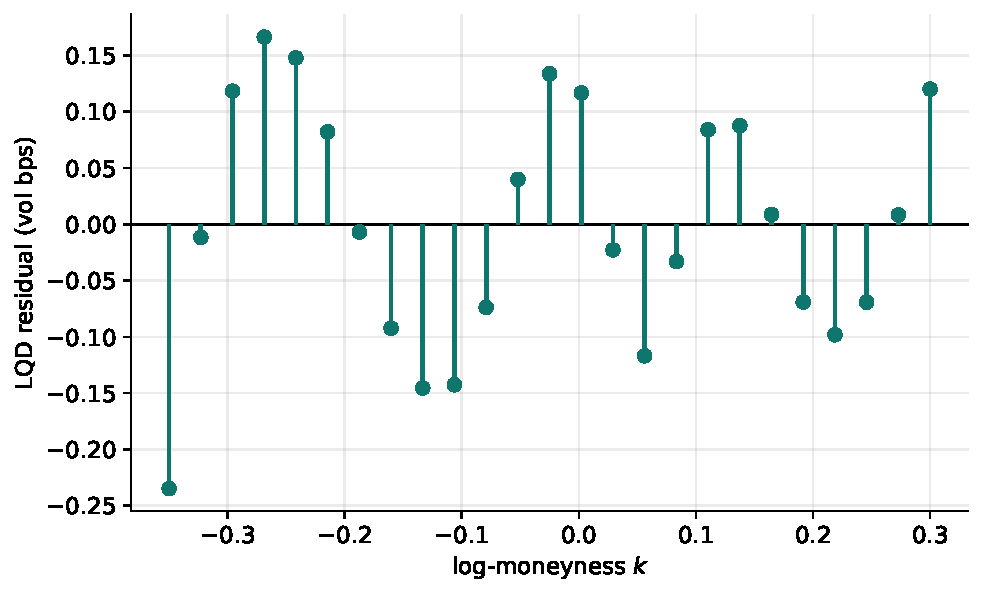
\includegraphics[width=\textwidth]{fig_lqd_svi_error.pdf}
\end{minipage}
\caption{Left: the SVI-JW target, the seven-parameter LQD fit, and the quotes.
Right: the LQD implied-volatility residual at the quotes, in volatility basis
points. Beyond the calibration window the LQD curve is its own Lee-consistent
extrapolation, not an SVI continuation.}
\label{fig:svi}
\end{figure}

\begin{figure}[H]
\centering
\begin{minipage}{0.49\textwidth}\centering
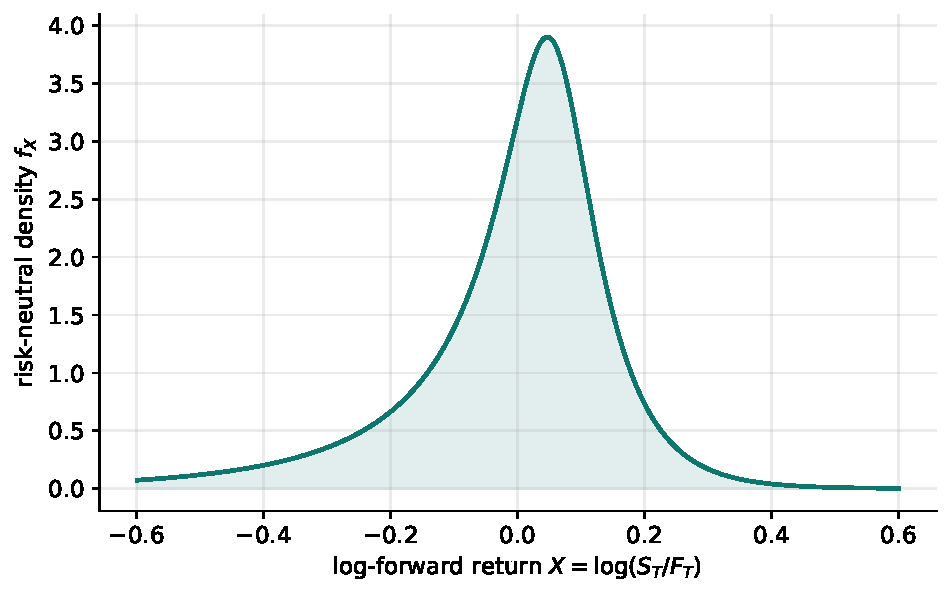
\includegraphics[width=\textwidth]{fig_lqd_density.pdf}
\end{minipage}\hfill
\begin{minipage}{0.49\textwidth}\centering
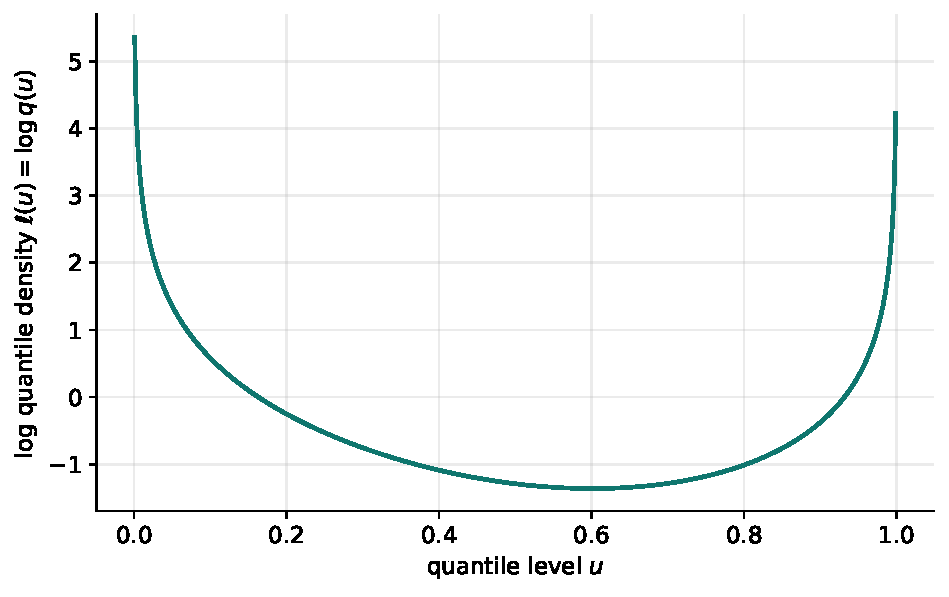
\includegraphics[width=\textwidth]{fig_lqd_logq.pdf}
\end{minipage}
\caption{Left: the risk-neutral log-return density of the LQD slice fitted to
the SVI target --- non-negative by construction. Right: the fitted log quantile density
$\ell(u)=\log q(u)$; the $-\log u-\log(1-u)$ endpoints are the source of the
exponential tails.}
\label{fig:density}
\end{figure}

\begin{table}[H]
\centering
\caption{Seven-parameter LQD fit to the SPX-like SVI-JW slice (fresh run).}
\label{tab:svi_coeffs}
\lqdsvicoefftable
\end{table}

\subsection{A bimodal ``double-hat'' event smile}

Ahead of a scheduled binary event the terminal density can be \emph{bimodal}, a
shape a low-order direct-IV model fights. The target here is an equal mixture of
two log-return normals with $\sigma=5\%$ centred near $\pm9$--$10\%$ over
$T=30/365$, martingale-normalized. A thirteen-parameter $N=12$ LQD fit over
$k\in[-0.25,0.25]$ recovers both the smile and the two-humped density
(\cref{fig:doublehat}), with endpoint scales $A_L=\lqddhAL$, $A_R=\lqddhAR$ and a
maximum implied-volatility error of \lqddhmaxerr\ volatility basis points.
Positivity of the density is automatic even where the higher Legendre modes
sculpt the two hats; in a sparse market one would lean on the ridge or the
ATM-orthogonal chart to avoid spurious oscillation.

\begin{figure}[H]
\centering
\begin{minipage}{0.49\textwidth}\centering
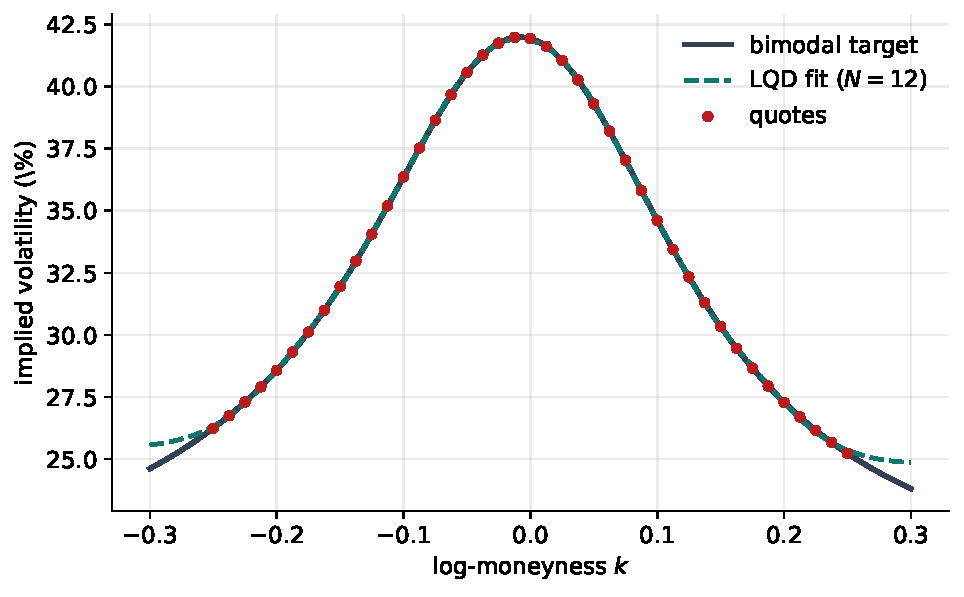
\includegraphics[width=\textwidth]{fig_lqd_doublehat.pdf}
\end{minipage}\hfill
\begin{minipage}{0.49\textwidth}\centering
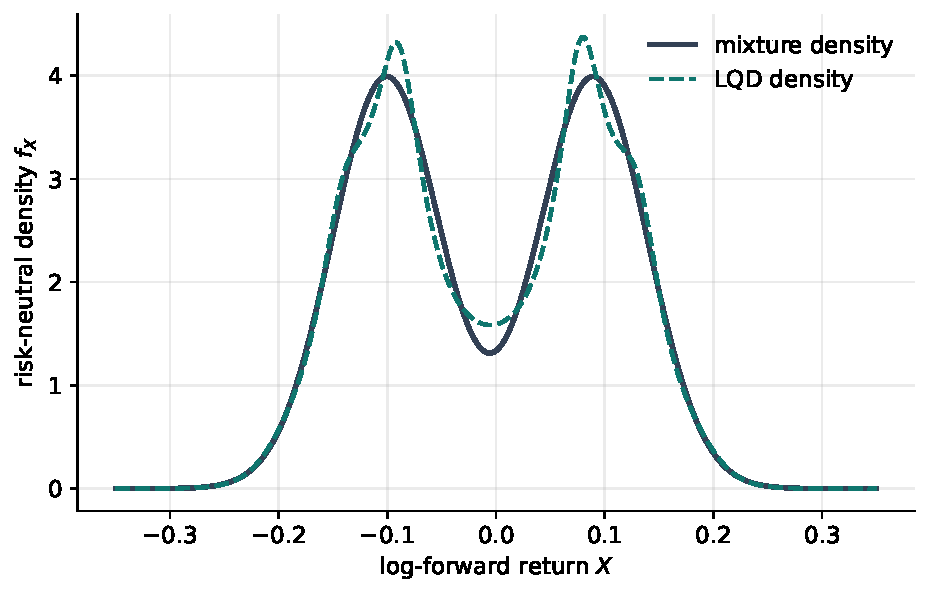
\includegraphics[width=\textwidth]{fig_lqd_doublehat_dens.pdf}
\end{minipage}
\caption{The bimodal event example. Left: target smile and $N=12$ LQD fit ---
note the central trough and supported wings that a quadratic-in-$k$ model cannot
make. Right: the true mixture density and the LQD density, both with two hats.}
\label{fig:doublehat}
\end{figure}

%======================================================================
\section{What is genuinely original here}
\label{sec:original}

Quantile-based and density-based smile constructions are not new, and the Lee
analysis is classical. Three things in this implementation are worth singling
out:
\begin{enumerate}[leftmargin=1.6em]
\item \textbf{The endpoint basis $-\log u-\log(1-u)+(1-u)L+uR$.} It is what makes
the tails \emph{exponential with controllable scale} while keeping the body in a
clean orthogonal-polynomial space; the Lee slopes \eqref{eq:lee_slopes} then come
out of the parametrization rather than being patched on.
\item \textbf{The exact ATM handles and the orthogonal chart}
(\cref{sec:atm}). The level/skew/curvature are closed-form functionals of the
quantile, so the model carries genuine trader coordinates \emph{and} a chart in
which the optimizer's shape modes do not disturb them --- the same three handles
that the graph extrapolator propagates in Note~14.
\item \textbf{The implicit-root cancellation} (\cref{thm:cancel}). The strike
root's dependence on $\theta$ vanishing from the price gradient is what turns a
$P+1$-rebuild finite-difference Jacobian into a one-pass analytic one; the
benchmark reaches the same fitted solution within the stated tolerance.
\end{enumerate}

%======================================================================
\section{Limitations}
\label{sec:limits}

LQD removes butterfly arbitrage by construction but \emph{not} calendar
arbitrage across independently fitted expiries --- and the cross-expiry
machinery of \cref{sec:calendar} is \emph{soft}, finite-weight and optional,
so a coupled surface is calendar-\emph{controlled}, not calendar-guaranteed.
Very high Legendre orders can fit noise and sculpt spurious density wiggles;
this is a model-risk, not an arbitrage, problem, controlled by the ridge,
bid--ask weighting and event priors. Several further limits deserve explicit
statement:
\begin{itemize}[leftmargin=1.4em]
\item \textbf{Near the integrability wall.} As $A_R\to1$ the forward integral
degenerates: the tail corrections dominate, conditioning of the fit and of the
retarget Newton solve deteriorates, and the barrier is doing real work. Fits
that live near the wall should be treated as fragile even when admissible.
\item \textbf{Atoms of any kind.} The model is a continuous law on
$(0,\infty)$: not only a jump-to-default atom at zero but \emph{any} exact
mass point (e.g.\ a pinned settlement price) can only be approximated by a
sharp continuous feature, never represented.
\item \textbf{Positive is not plausible.} Structural positivity guarantees a
\emph{density}, not a sensible one: an unregularized high-order fit can
produce economically implausible (multi-modal, spiky) yet perfectly
arbitrage-free shapes. Positivity removes one failure class; judgment and the
ridge handle the rest.
\item \textbf{Coefficient non-uniqueness in practice.} Distinct coefficient
vectors can price indistinguishably (near-degenerate directions grow with $N$
and with sparse data), so fitted coefficients are not comparable across fits
--- compare handles, curves and densities, not raw $\theta$.
\item \textbf{Unstudied sensitivities.} There is no dedicated study of
handle \emph{drift} under rolling recalibration, nor of digital/one-touch
sensitivities to the interpolation scheme; both are open measurement items,
not established properties.
\end{itemize}

%======================================================================
\section{Traceability}
\label{sec:traceability}

One caveat on the ``match note'' anchors: the fixture coefficients those tests
lock were recorded when the benchmark was first frozen, so they are
\emph{legacy locks} --- they pin the production behaviour against regression,
but their literal values can lag the freshly regenerated tables in this note
(the note's numbers always come from a fresh \texttt{gen\_lqd.py} run). Where
the two disagree, the fresh run is the current truth and the test is the
regression tripwire.

\begingroup
\small
\setlength{\tabcolsep}{4pt}
\renewcommand{\arraystretch}{1.15}
\begin{longtable}{@{}p{0.30\textwidth}p{0.11\textwidth}p{0.55\textwidth}@{}}
\caption{Claims in this note and the code/tests that lock them.}\\
\toprule Claim & Object & Code anchor \newline \emph{Test anchors}\\ \midrule
\endfirsthead
\toprule Claim & Object & Code anchor \newline \emph{Test anchors}\\ \midrule
\endhead
Density positive; call curve monotone and convex; parity holds &
\cref{prop:nobutterfly} &
\nolinkurl{models/lqd/quadrature.py}\newline
\nolinkurl{test_lqd_pricing.py::test_density_positive}\newline
\nolinkurl{::test_call_curve_monotone_and_convex_in_strike}\newline
\nolinkurl{::test_put_call_parity}\\
\addlinespace
Martingale shift correct; $\E[e^X]=1$ &
\eqref{eq:mu_norm} &
\nolinkurl{models/lqd/quadrature.py}\newline
\nolinkurl{test_lqd_pricing.py::test_svi_fit_martingale_shift_matches_note}\newline
\nolinkurl{::test_svi_fit_martingale_integral_is_one}\\
\addlinespace
Endpoint scales and Lee slopes; stable for extreme scales &
\eqref{eq:AL}--\eqref{eq:lee_slopes} &
\nolinkurl{models/lqd/basis.py}\newline
\nolinkurl{test_lqd_basis.py::test_svi_fit_endpoint_scales_match_note}\newline
\nolinkurl{::test_svi_fit_lee_slopes_match_note}\newline
\nolinkurl{::test_lee_slopes_stable_for_tiny_nonzero_endpoint_scales}\\
\addlinespace
Legendre basis: recursion and orthogonality &
\eqref{eq:leg_recursion} &
\nolinkurl{models/lqd/basis.py}\newline
\nolinkurl{test_lqd_basis.py::test_legendre_recursion_matches_explicit_polynomials}\newline
\nolinkurl{::test_legendre_orthogonality_on_unit_interval}\\
\addlinespace
Exact ATM handles &
\eqref{eq:atm_handles} &
\nolinkurl{models/lqd/atm.py}\newline
\nolinkurl{test_lqd_atm.py::test_atm_level_matches_implied_vol}\newline
\nolinkurl{::test_atm_skew_matches_finite_difference}\newline
\nolinkurl{::test_atm_curvature_matches_finite_difference}\\
\addlinespace
Orthogonal chart: shape moves preserve handles; retarget exact &
\cref{sec:ortho} &
\nolinkurl{models/lqd/ortho.py}\newline
\nolinkurl{test_lqd_ortho.py::test_shape_move_leaves_handles_nearly_unchanged}\newline
\nolinkurl{::test_retarget_hits_exact_handles}\\
\addlinespace
Analytic Jacobian matches FD (mid, band, calendar); fits agree &
\cref{thm:cancel} &
\nolinkurl{models/lqd/jacobian.py}\newline
\nolinkurl{test_lqd_jacobian.py::test_jacobian_matches_fd_mid}\newline
\nolinkurl{::test_jacobian_matches_fd_band}\newline
\nolinkurl{::test_jacobian_matches_fd_calendar}\newline
\nolinkurl{::test_analytic_and_fd_fits_agree}\\
\addlinespace
Barrier finite for wild trial parameters &
\eqref{eq:barrier} &
\nolinkurl{models/lqd/calibrate.py}\newline
\nolinkurl{test_lqd_jacobian.py::test_barrier_residual_finite_for_wild_tail_scale}\\
\addlinespace
Benchmark fit and speed rail (legacy fixture) &
\cref{sec:examples} &
\nolinkurl{models/lqd/calibrate.py}\newline
\nolinkurl{test_lqd_calibrate.py::test_calibrate_to_svi_benchmark}\newline
\nolinkurl{::test_calibration_is_fast_enough}\\
\addlinespace
Double-hat event smile: bimodal density recovered &
\cref{sec:examples} &
\nolinkurl{models/lqd/calibrate.py}\newline
\nolinkurl{test_lqd_pricing.py::test_double_hat_density_is_bimodal}\\
\addlinespace
JW conversion used by the benchmark &
\cref{app:svijw} &
\nolinkurl{models/svi_jw/svi.py}\newline
\nolinkurl{test_lqd_pricing.py::test_jw_conversion_matches_note}\\
\bottomrule
\end{longtable}
\endgroup

\appendix
%======================================================================
\section{LQD-native controls and numerical constants}
\label{app:atlas}

The knobs \emph{specific to} the LQD slice, with defaults and roles. Surfaced
knobs are user-facing \texttt{FitSettings}; hidden knobs are internal constants
tuned to the algorithm and not exposed. The \emph{shared} calibration controls
that also shape an LQD fit --- \texttt{fitMode}, \texttt{haircut},
\texttt{midAnchorWeight}, \texttt{enforceCalendar}/\texttt{calendarWeight},
the var-swap controls, and the prior-persistence and observation-filter
settings of \cref{tab:stack} --- are indexed in Note~00's control table and
derived in their own notes (07, 08, 10, 13, 15); they are deliberately not
duplicated here.

\begin{longtable}{p{0.26\textwidth}p{0.12\textwidth}p{0.54\textwidth}}
\caption{LQD-native controls.}\label{tab:atlas}\\
\toprule
Knob & Default & Role\\
\midrule
\endfirsthead
\toprule Knob & Default & Role\\ \midrule
\endhead
\multicolumn{3}{l}{\emph{Surfaced (FitSettings)}}\\
\midrule
\texttt{nOrder} $N$ & $6$ & Legendre expansion order; $7$ parameters at $N=6$.
Schema range $4\le N\le16$: $6$ for ordinary slices, $8$--$14$ for
scheduled-event slices.\\
\texttt{regLambda} $\lambda$ & $10^{-6}$ & High-order ridge coefficient in
\eqref{eq:calib_objective}; suppresses oscillation in sparse data.\\
\texttt{regPower} $r$ & $1.0$ & Ridge exponent in $n^{2r}a_n^2$; larger $r$
penalizes high modes harder.\\
\texttt{barrierCenter} $c$ & \lqdbarriercenter & Centre of the $A_R$ softplus
barrier \eqref{eq:barrier}; engages before the $A_R=1$ wall.\\
\texttt{barrierScale} $s$ & \lqdbarrierscale & Steepness of that barrier.\\
\texttt{weightScheme} & \texttt{equal} & Per-quote weights $\omega_i$
(\texttt{equal} or \texttt{tv\_density}); see Note~07.\\
\midrule
\multicolumn{3}{l}{\emph{Hidden (internal constants)}}\\
\midrule
\texttt{Z\_MAX} $Z$ & $40.0$ & Half-width of the symmetric logit quadrature grid;
truncation error $\ll$ vega noise for equity tails.\\
\texttt{N\_POINTS} & $8001$ & Reporting/diagnostic grid nodes (odd, so $z=0$ is a
node).\\
\texttt{OPT\_N\_POINTS} & \lqdoptpts & Coarser grid used during the
optimization iterations; accepted slice rebuilt at \texttt{N\_POINTS}.\\
\texttt{EPS\_AR} $\eps_R$ & $10^{-6}$ & Buffer in the hard bound $A_R<1-\eps_R$.\\
\texttt{\_VEGA\_FLOOR} $\eta$ & $10^{-4}$ & Floor added to Black vega in the
residual normalization \eqref{eq:vega_resid}.\\
\texttt{xtol/ftol/gtol} & $10^{-10}$ & \texttt{trf} tolerances; $\sim6$ orders
below the fit budget, so the optimum is display-identical while \texttt{trf}
stops grinding invisible reductions.\\
\texttt{max\_nfev} & $4000$ & Evaluation cap (rarely approached).\\
\bottomrule
\end{longtable}

%======================================================================
\section{Performance notes}
\label{app:perf}

\begin{enumerate}[leftmargin=1.6em]
\item \textbf{Cached static grid.} The grid $(z,u,u(1-u))$ and the Legendre
matrix depend only on $(Z,n_{\text{pts}},N)$, so they are LRU-cached and returned
read-only; only $g(u)$ is re-formed per call. This removed $\sim40\%$ of
\texttt{build\_slice} and made each build $\sim1.7\times$ faster.
\item \textbf{Two-grid optimization.} Iterations run on \texttt{OPT\_N\_POINTS}
$=\lqdoptpts$ (Simpson error already far below the fit budget); the accepted
slice is rebuilt once at $8001$ nodes for the reported result, density, var-swap
and calendar diagnostics. Converged parameters agree with a full-grid fit to
$\sim10^{-6}$.
\item \textbf{Hermite interpolation/inversion.} Storing the exact nodal
derivatives $\dd Q/\dd z$ and $\dd A/\dd z$ gives cubic-Hermite off-grid
evaluation (clean Greeks) and machine-precision strike inversion by
Hermite--Newton --- and supplies precisely the nodal sensitivities the analytic
Jacobian reuses.
\item \textbf{Analytic Jacobian} (\cref{sec:jacobian}). One quadrature pass
instead of $P+1$ finite-difference rebuilds, reaching the same fitted solution
within tolerance (relative cost agreement $\sim10^{-11}$), measured
$1.3$--$1.7\times$ on the residual-path benchmark of \cref{tab:timing} and
structurally more on heavier configurations. Gated to the var-swap/prior-free
configuration.
\item \textbf{Looser tolerances.} Dropping \texttt{trf} tolerances from
$10^{-15}$ to $10^{-10}$ stops the optimizer chasing a $10^{-15}$ cost reduction
that is invisible in the priced surface, saving whole $(P+1)$-eval iterations at
no display-precision cost.
\end{enumerate}

%======================================================================
\section{The SVI-JW conversion used in the example}
\label{app:svijw}

SVI (``stochastic volatility inspired'') is the five-parameter total-variance
slice $w(k)=a+b\{\rho(k-m)+\sqrt{(k-m)^2+\sigma_{\mathrm{SVI}}^2}\}$; SVI-JW
(``jump-wings'') re-coordinatizes it into trader quantities. The JW parameters
$(v,\psi,p,c,\widetilde v)$ relate to raw SVI by
$w_0=vT$, $b=\tfrac{\sqrt{w_0}}{2}(p+c)$, $\rho=\tfrac{c-p}{c+p}$,
$\psi=\tfrac{b}{2\sqrt{w_0}}\big(\rho-\tfrac{m}{\sqrt{m^2+\sigma_{\mathrm{SVI}}^2}}\big)$ and
$\widetilde vT=a+b\sigma_{\mathrm{SVI}}\sqrt{1-\rho^2}$. Setting
$\chi=\tfrac{m}{\sqrt{m^2+\sigma_{\mathrm{SVI}}^2}}=\rho-\tfrac{4\psi}{p+c}$ gives
$m=\chi\sigma_{\mathrm{SVI}}/\sqrt{1-\chi^2}$ and
$\sqrt{m^2+\sigma_{\mathrm{SVI}}^2}=\sigma_{\mathrm{SVI}}/\sqrt{1-\chi^2}$,
and subtracting the minimum-variance relation from the ATM relation,
\begin{equation}
\sigma_{\mathrm{SVI}}=\frac{w_0-\widetilde vT}{b\big((1-\rho\chi)/\sqrt{1-\chi^2}-\sqrt{1-\rho^2}\big)},
\quad m=\frac{\chi\sigma_{\mathrm{SVI}}}{\sqrt{1-\chi^2}},
\quad a=\widetilde vT-b\sigma_{\mathrm{SVI}}\sqrt{1-\rho^2}.
\end{equation}
The inversion is exact on its documented domain --- $p+c>0$, $|\chi|<1$ and a
nonzero denominator above --- and has a genuine \emph{coordinate singularity}
at $\psi=0$ with $m\ne0$ handled separately (Note~02 states the full domain
contract, $-p/2<\psi<c/2$, and its $\psi=0$ stratum). The benchmark's raw
parameters in \cref{sec:examples} are the image, at $T=0.5$, of
\[
(v,\psi,p,c,\widetilde v)=(0.0425,\,-0.25,\,0.75,\,0.25,\,0.034).
\]

%======================================================================
\section{Reference implementation}
\label{app:ref}

The whole slice is one quadrature pass in the logit coordinate $z=\log(u/(1-u))$:
form $g$, integrate $\dd Q/\dd z=e^{g}$ to the quantile, solve one scalar
normalization for the martingale shift $\mu$, and reverse-integrate the
asset-share $A(z)$; every strike is then priced by $C(k)=A(z_k)-e^k(1-u_k)$. The
listing below reproduces \texttt{build\_slice}'s quantile, asset share and $\mu$ to
$10^{-8}$ on the $N=6$ benchmark and gives $\E[e^X]=1.000000$ (production inverts
$Q(z_k)=k$ and interpolates $A$ with cubic Hermite for smooth Greeks; the linear
\texttt{np.interp} here agrees to $10^{-7}$ on the dense grid).

\begin{lstlisting}[caption={The LQD quadrature pipeline (distilled from
\texttt{models/lqd/\{basis,quadrature\}.py}).}]
def legendre(n_max, x):            # P_0..P_{n_max}, 3-term recursion
    P = np.empty((n_max+1, x.size)); P[0] = 1.0; P[1] = x
    for n in range(1, n_max):
        P[n+1] = ((2*n+1)*x*P[n] - n*P[n-1]) / (n+1)
    return P

def g_of_u(u, L, R, a):            # smooth part g(u) of ell(u)
    return (1-u)*L + u*R + a @ legendre(len(a)+1, 1 - 2*u)[2:]

def build_slice(z, L, R, a):
    # One quadrature pass, eqs (q_logit)-(mu_norm).
    u = expit(z); dz = z[1] - z[0]
    # Tail scales e^{g(0)}, e^{g(1)}:
    A_L, A_R = np.exp(g_of_u(np.array([0.0, 1.0]), L, R, a))
    dQ = np.exp(g_of_u(u, L, R, a))          # dQ/dz = e^{g}
    Q = cumulative_simpson(dQ, dx=dz, initial=0.0)
    Q -= Q[len(z)//2]                        # anchor Q(0) = 0
    mass = np.exp(Q)*u*(1-u)
    tot = (np.trapezoid(mass, z)             # + analytic tails
           + np.exp(Q[-1]-z[-1])/(1-A_R)
           + np.exp(Q[0]-z[-1])/(1+A_L))
    mu = -np.log(tot); Q = Q + mu            # now E[e^X] = 1
    m = np.exp(Q)*u*(1-u)
    # Asset share A(z) = int_z^inf e^{Q} u(1-u):
    A = (cumulative_simpson(m[::-1], dx=dz, initial=0.0)[::-1]
         + np.exp(Q[-1]-z[-1])/(1-A_R))
    return u, Q, A

def call_price(k, z, u, Q, A):
    # C(k) = A(z_k) - e^k (1 - u_k)
    zk = np.interp(k, Q, z)                  # invert Q(z_k) = k
    return np.interp(zk, z, A) - np.exp(k)*(1 - expit(zk))
\end{lstlisting}

\begin{thebibliography}{9}
\bibitem{BreedenLitzenberger1978} D.~Breeden and R.~Litzenberger.
Prices of state-contingent claims implicit in option prices.
\emph{Journal of Business}, 51(4):621--651, 1978.
\bibitem{Lee2004} R.~W.~Lee.
The moment formula for implied volatility at extreme strikes.
\emph{Mathematical Finance}, 14(3):469--480, 2004.
\bibitem{Gatheral2006} J.~Gatheral.
\emph{The Volatility Surface: A Practitioner's Guide}. Wiley, 2006.
\bibitem{GatheralJacquier2014} J.~Gatheral and A.~Jacquier.
Arbitrage-free SVI volatility surfaces.
\emph{Quantitative Finance}, 14(1):59--71, 2014.
\bibitem{Strassen1965} V.~Strassen.
The existence of probability measures with given marginals.
\emph{Annals of Mathematical Statistics}, 36(2):423--439, 1965.
\bibitem{CarrMadan1998} P.~Carr and D.~Madan.
Towards a theory of volatility trading.
In \emph{Volatility}, Risk Books, 1998.
\end{thebibliography}

\end{document}
